\documentclass[10pt]{article}
\usepackage{listings}
\usepackage{graphicx}
\addtolength{\oddsidemargin}{-.875in}
	\addtolength{\evensidemargin}{-.875in}
	\addtolength{\textwidth}{1.75in}

	\addtolength{\topmargin}{-.875in}
	\addtolength{\textheight}{1.75in}
\renewcommand{\baselinestretch}{0.97}
\title{Assignment 1}
\author {Suraj S, 2018MCS2024}

\begin{document}

\maketitle

The Assignments were made on python2 

\section{Linear Regression}
\subsection{Implementing the batch gradient descent}
The batch gradient descent was implemented in the following section used the following equations in order to implement the batch gradient descent.
\\

\begin{itemize}
\item the cost function
$$\displaystyle J(\theta)= \frac{1}{2m}\sum_{i=1}^{m} \left(h_{\theta}(x^{(i)})-y^{(i)}\right)^2$$
\item gradient descent for the $j^{th}$ theta parameters 
$$\displaystyle \theta_j:=\theta_j-\alpha\frac{\partial}{\partial\theta_j}J(\theta)\mbox{ for j=0,1...n}$$
for j=1 can be further rewritten as :$\displaystyle \frac{\partial}{\partial\theta_1}\left(\frac{1}{2m}\sum_{i=1}^{m} \left(\theta_0+\theta_1x^{(i)}-y^{(i)}\right)^2 \right) = \frac{1}{m}\sum_{i=1}^{m} \left(\theta_0+\theta_1x^{(i)}-y^{(i)}\right).x^{(i)} = \frac{1}{m}\sum_{i=1}^{m} \left(h_{\theta}(x^{(i)})-y^{(i)}\right).x^{(i)}$
\end{itemize}
now implementing the gradient descent,we have first normalized the data in order to have mean 0 and variance 1 
\\
using the gradient descent we have the used the convergence condition as the difference between the initial and final cost should be less than a given a threshold(i.e about $10^{-9}$ )
\\
\\
the following output was given by the program upon convergence

\begin{lstlisting}
Converged
Following are the details of the gradient descent
Learning Rate: 0.1
Stopping Criteria:absolute value of difference between the initial and final error
The number of iterations took in order to converge is 29
Theta Values(Final Parameters) [[0.99653574 0.00134008]]
\end{lstlisting}
\newpage
\subsection{Plotting the line}
the lines were plotted using the value of $\eta=$ 0.1
\\
\begin{center}
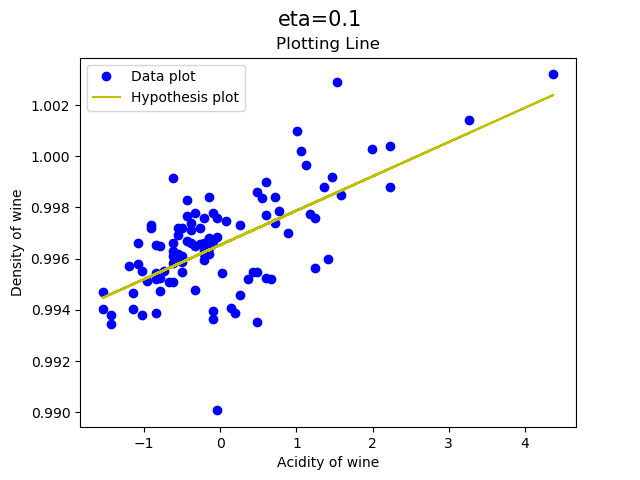
\includegraphics[scale=0.4]{linearplot01.png} 
\end{center}
\subsection{Plotting the mesh}
the mesh were plotted using the value of $\eta=$ 0.1
\\
\begin{center}
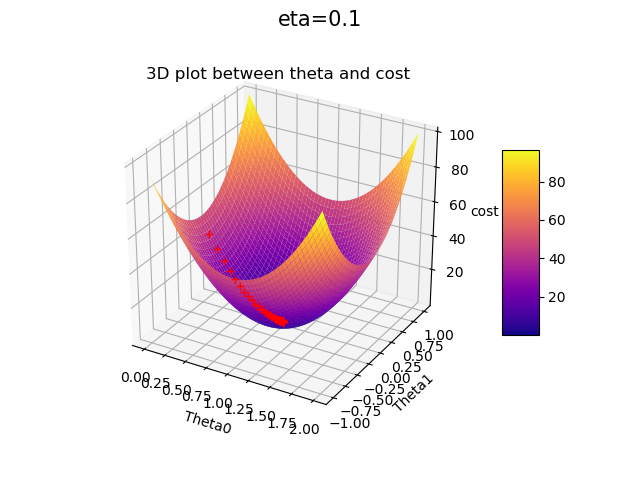
\includegraphics[scale=0.8]{meshplot01.png} 
\end{center}
\newpage
\subsection{Plotting the contours}
the contour were plotted using the value of $\eta=$ 0.1
\\
\begin{center}
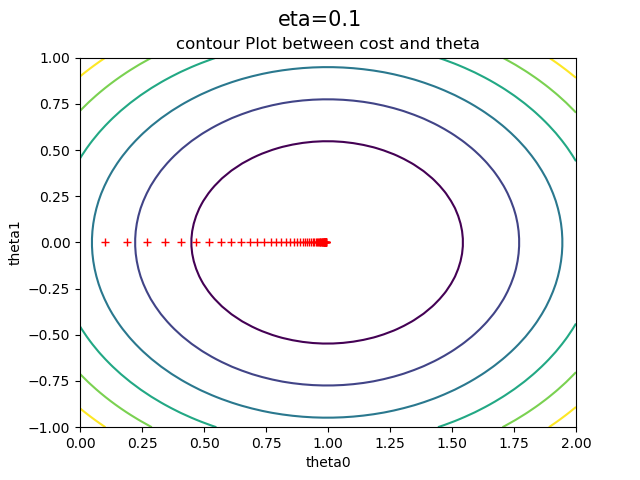
\includegraphics[scale=0.8]{contourplot01.png} 
\end{center}

\subsection{trying with different values of $\eta$}
In this section we have used the various values of $\eta=\{0.1,0.5,0.9,1.3,1.7,2.1,2.4,2.9\}$ and ran the above procedure with these values we have noticed that the gradiend descent didn't converged in the 
value from 2.1 also we have noticed that the number of iterations that was required for the convergence was reduced as the value was increased.
\\
\newpage
\section{Locally Weighted Linear regression}
The data was first normalized and then the data was processed further

The normal equations in order to find the parameters used in the following sections are as follows:
\\
\\
For unweighted linear regression:
$$\theta=(X^TX)^{-1}X^TY$$
\\
\\
For locally weighted linear regression:
$$\theta=(X^TWX)^{-1}X^TWY$$

\subsection{Unweighted Linear Regression}
In this section we have implemented the unweighted linear regression for the distribution.
\begin{center}
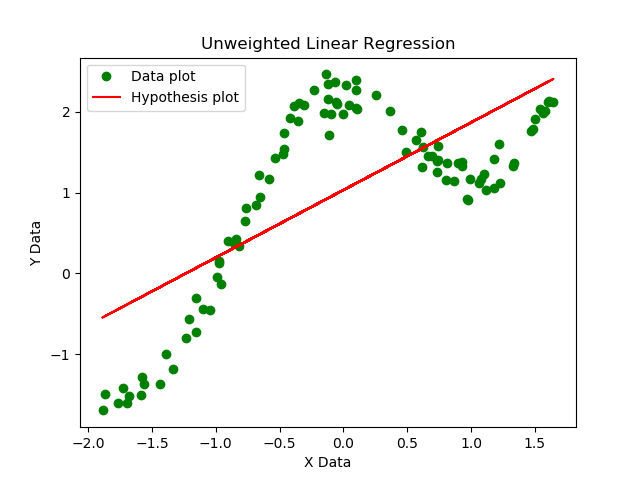
\includegraphics[scale=0.8]{wlinearplot.png} 
\end{center}
\newpage
\subsection{Locally Weighted Linear Regression}
In this section we have implemented the weighted linear regression for the distribution using the value of $\tau=0.8$.
  
\begin{center}
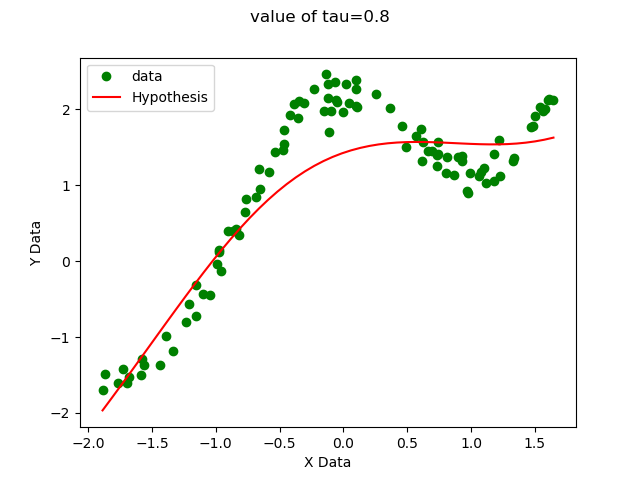
\includegraphics[scale=0.8]{weightedt08.png} 
\end{center} 
\newpage
\subsection{Weighted Linear Regression using different $\tau$}
In this section we have implemented the weighted linear regression for the distribution using different values of $\tau$, the values of $\tau$ used are $\{0.1, 0.3, 2,10\}$ we can see that as we increase the value of $\tau$ the locally weighted linear regression tends to become linear regression.
\\
\\
Also if we take the value of $\tau$ too large it might underfit the curve and might can act like the linear regression and if we take the value of $\tau$ to be small it is likely to overfit the data
\begin{center}
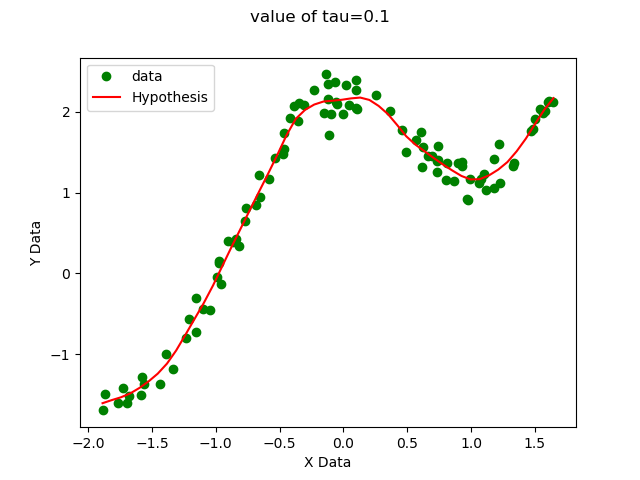
\includegraphics[scale=0.8]{weightedt01.png} 
\end{center} 
\begin{center}
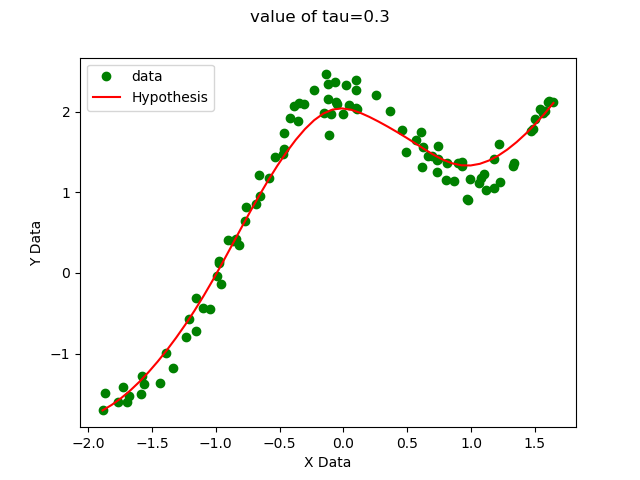
\includegraphics[scale=0.8]{weightedt03.png} 
\end{center} 
\begin{center}
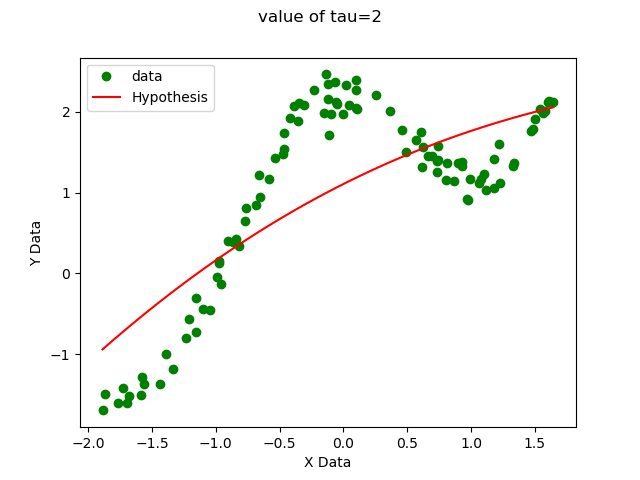
\includegraphics[scale=0.8]{weightedt2.png} 
\end{center} 
\begin{center}
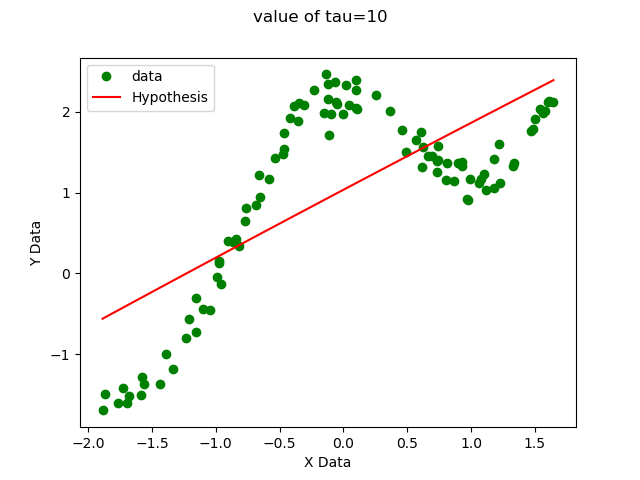
\includegraphics[scale=0.8]{weightedt10.png} 
\end{center}
\newpage 
\section{Logistic Regression}
The data was first normalized and then the data was processed further
\subsection{Newton's method}
In this section we have implemented the logistic regression for the distribution for classifying the two element using the newton's method to find the parameters.
\begin{lstlisting}
Following are the details of the Newton's method

Stopping Criteria:absolute value of difference between the initial and final 
error

Theta Values(Final Parameters) 
[[ 0.40125316]
 [ 2.5885477 ]
 [-2.72558849]]

No.of iterations:7
\end{lstlisting}
\subsection{Graph plot}
\begin{center}
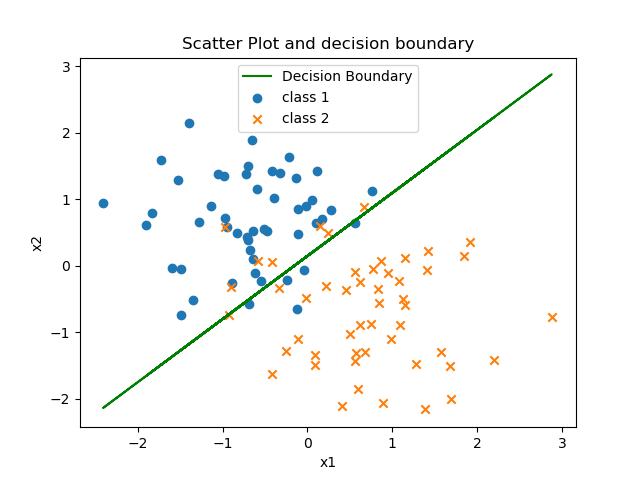
\includegraphics[scale=0.8]{newton.png} 
\end{center} 
\newpage
\section{Gaussian Discriminant Analysis}
The data was first normalized and then the data was processed further
\subsection{various values of the parameters:}
The values of the various parameters are given below:
\begin{itemize}
\item $\mu_0=$[-0.75529433  0.68509431]
\item $\mu_1=$[0.75529433  -0.68509431]
\item $\Sigma=$
[[ 0.42953048 -0.02247228]
 [-0.02247228  0.53064579]]
\item $\phi=$0.5
\end{itemize}
\subsection{data plot for points}
\begin{center}
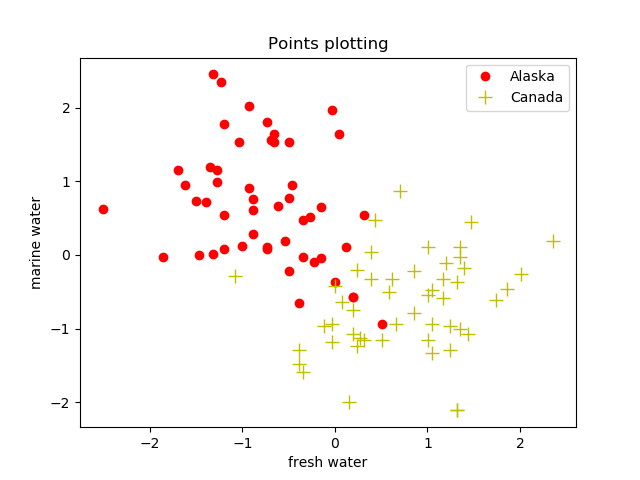
\includegraphics[scale=0.8]{pointplot.png} 
\end{center}
\newpage
\subsection{data plot for linear speration using same covariance matrix}
\begin{center}
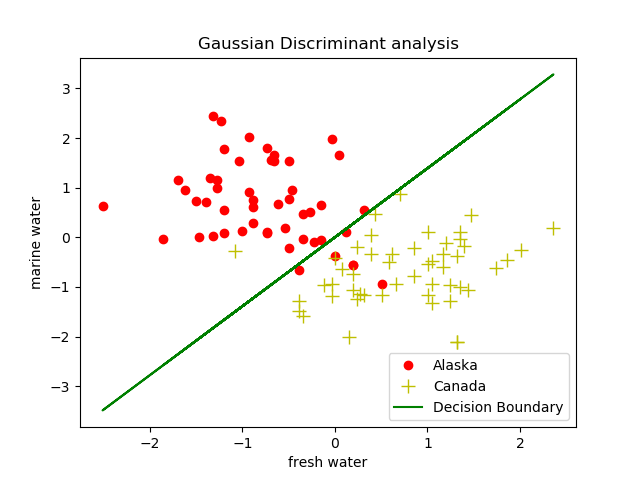
\includegraphics[scale=0.8]{gline.png} 
\end{center}
\subsection{various values for differrent covariance matrix}
The values of the various parameters are given below:
\begin{itemize}
\item $\mu_0=$[-0.75529433  0.68509431]
\item $\mu_1=$[0.75529433  -0.68509431]
\item $\Sigma_0=$[[ 0.38158978 -0.15486516]
 [-0.15486516  0.64773717]]
\item $\Sigma_1=$[[0.47747117 0.1099206 ]
 [0.1099206  0.41355441]]
\item $\phi=$0.5
\end{itemize} 
\subsection{data plot for linear separation using same covariance matrix}
\begin{center}
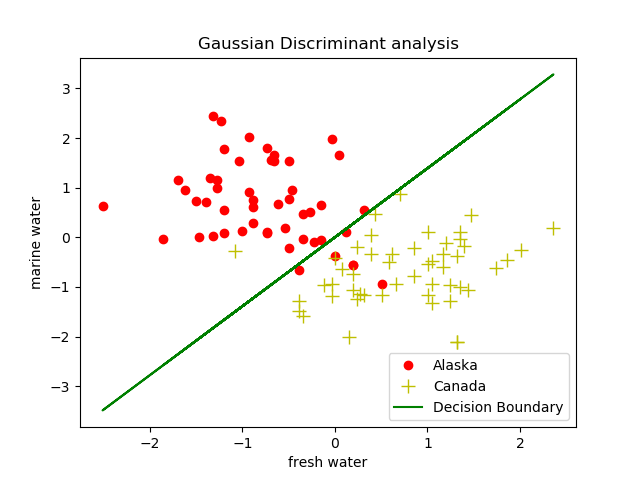
\includegraphics[scale=0.8]{gline.png} 
\end{center}
\subsection{linear along with quadratic boundary}
\begin{center}
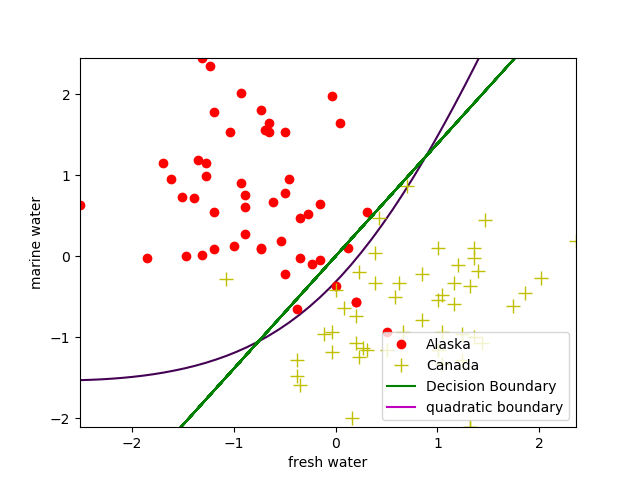
\includegraphics[scale=0.8]{gaussianwline.png} 
\end{center}
\end{document}

